% !TeX program = lualatex
% !TeX encoding = utf8
% !TeX spellcheck = uk_UA
% !BIB program = bibler

\documentclass{beamer}
\usetheme{Electromagnetism}
\usepackage{Electromagnetism}
\usetikzlibrary{spy}
\hypersetup{
  colorlinks=true,
  linkcolor=cyan,  % Цвет для внутренних ссылок
  urlcolor=red,    % Цвет для URL
  citecolor=blue   % Цвет для библиографических ссылок
}




%============================================================================
\title[Лекції електрики та магнетизму]{\huge\bfseries Магнітне поле у вакуумі}
\subtitle{Лекції з електрики та магнетизму}
\author{Пономаренко С. М.}
\date{}
%============================================================================
\graphicspath{{pictures/}}

\begin{document}


\begin{frame}[plain]
	\maketitle
	%	\tikz[remember picture,overlay] \node[opacity=0.7,inner sep=0pt,
	%		anchor=north west] at (current page.north
	%	west){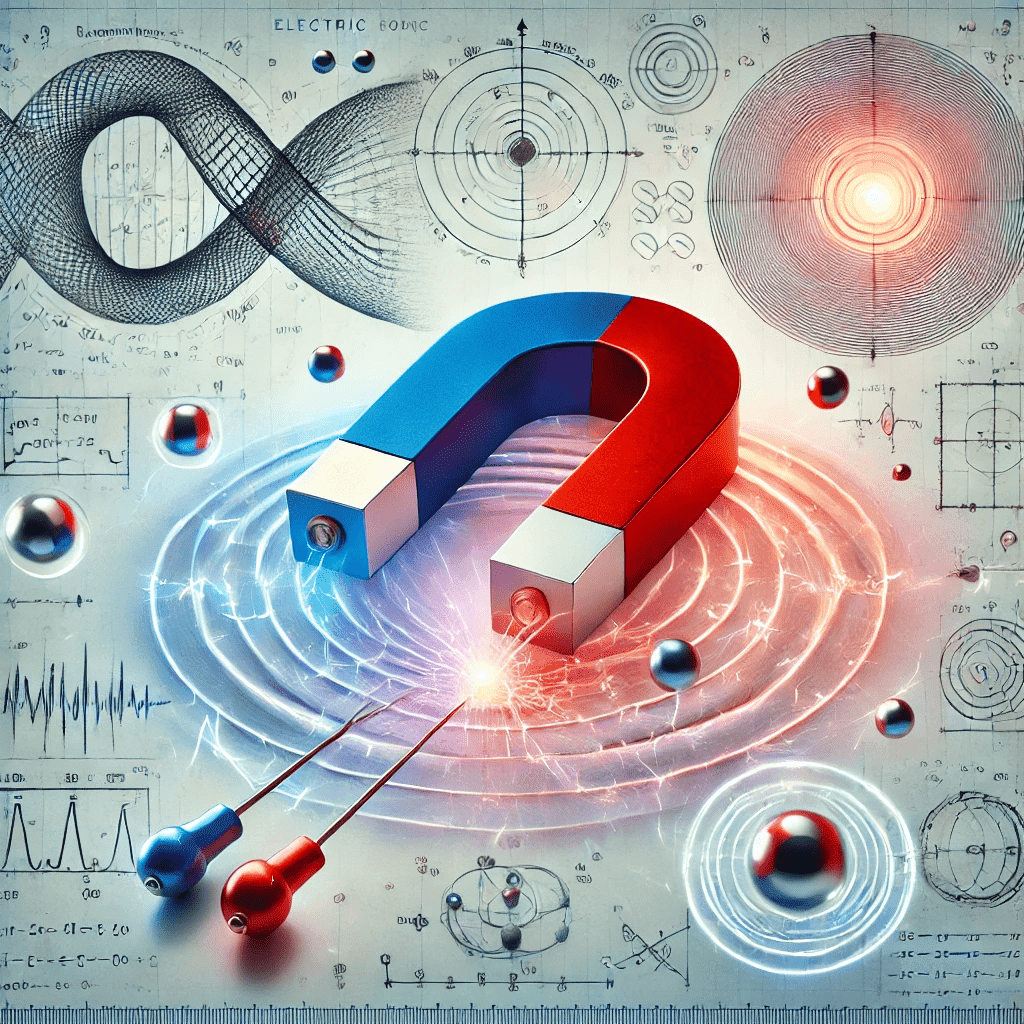
\includegraphics[width=2cm]{EMInteractions}};
\end{frame}

% ============================== Слайд ## ===================================
\begin{frame}{Зміст лекції}{}
	\tableofcontents
\end{frame}
% ===========================================================================

% ============================== Слайд ## ===================================
\begin{frame}{Означення}{}
	\begin{block}{}\justifying
		\alert{Магнітним полем} називається силове поле, що \alert{діє на рухомі заряди} і як наслідок --- на електричні струми  і на тіла, які мають
		магнітний  момент.

		\bigskip

		Магнітне поле створюється рухомими зарядами (електричним струмом). Незмінні в часі струми створюють постійні магнітні поля.
	\end{block}
\end{frame}
% ===========================================================================

% ============================== Слайд ## ===================================
\begin{frame}{Характеристика магнітного поля}{}\small
	\begin{block}{}\justifying
		Магнітних зарядів (магнітних монополів) у в природі немає (експериментальний факт). Характеристику магнітного поля, аналогічно до $\Efield =
			\frac{\vect{F}}{q}$
		ввести не можна. Однак в природі є магнітні диполі (магнітна стрілка, коловий виток зі струмом тощо), тому використовуючи аналогію з моментом
		сил, що діє на електричний диполь в електричному полі $ \vect{M} = \left[\vect{p}_e \times\Efield\right] $, можна ввести характеристику
		магнітного поля:
		\begin{equation*}
			\vect{M} = \left[\vect{p}_m \times\Bfield\right], \quad M_{\max} = p_m B
		\end{equation*}
		Характеристику магнітного поля, вектор $\Bfield$, по історичним причинам називають не \alert{напруженістю}, а \alert{індукцією} магнітного поля.
	\end{block}
	\begin{overprint}
		\onslide<1>
		\begin{block}{}\justifying
			Величина вектора індукції чисельно дорівнює максимальному обертальному моменту, що діє на одиничний магнітний момент вміщений у магнітне поле:
			\begin{equation*}
				B = \frac{\quad M_{\max}}{p_m}.
			\end{equation*}
		\end{block}
		\onslide<2>
		\begin{alertblock}{}\justifying
			В гауссовій системі одиниць величину магнітного поля називають Гаусом (Гс). С системі СІ Теслою (Тл):
			\begin{equation*}
				1\ \text{Тл} = 10^4\ \text{Гс}.
			\end{equation*}
		\end{alertblock}
	\end{overprint}
\end{frame}
% ===========================================================================

% ============================== Слайд ## ===================================
\begin{frame}{Сила Лоренца та сила Ампера}{}
	\begin{block}{}
		Магнітною складовою сили Лоренца називається сила, що діє на рухомий заряд $q$ з боку магнітного поля:
		\begin{equation*}
			\vect{F} = q\left[\frac{\vect{v}}{c}\times\Bfield\right].
		\end{equation*}
		Повна сила (власне і є сила Лоренца), що діє на заряд, включає також силу з боку електричного поля:
		\begin{equation*}
			\vect{F} = q\left( \Efield + \left[\frac{\vect{v}}{c}\times\Bfield\right] \right) .
		\end{equation*}
	\end{block}
	\begin{block}{}
		\alert{Силою Ампера} називають силу, що діє на струми з боку магнітного поля:
		\begin{equation*}
			d\vect{F} = \frac1c \left[ \vect{j}dV \times \Bfield\right],
		\end{equation*}
		де $\vect{j} dV$ --- називається об'ємним \alert{елементом струму}.
	\end{block}
\end{frame}
% ===========================================================================


% ============================== Слайд ## ===================================
\begin{frame}{Елемент струму}{}
	\begin{columns}
		\begin{column}{0.3\linewidth}\centering
			\begin{tikzpicture}[>=latex,
					spy using outlines={circle, magnification=3, size=3.2cm, connect spies}
				]
				\draw[gray!60, line width=0.21cm] (0,0)  [partial ellipse=90:0:2];
				\fill[gray!50, draw = gray!70] (0, 2) circle (0.05 and 0.1);
				\fill[gray!50, rotate=-90, draw = gray!70] (0, 2) circle (0.05 and 0.1);

				\draw[red!40, line width=0.21cm] (0,0) [partial ellipse=55:45:2];
				\draw[{Latex[scale=0.5]}-{Latex[scale=0.5]}] (55:2.2)  arc(55:45:2.1) node[above=-1pt, sloped, pos=0.7, font=\tiny] {$d\ell$};
				\fill[red!40, draw = red!60, rotate=-45] (0, 2) coordinate (S1) circle (0.05 and 0.1);
				\fill[red!40, draw = red!60, rotate=-35] (0, 2)  circle (0.05 and 0.1);

				\node[font=\tiny, right, inner sep=0] (S) at (42:2.2) {$S$};

				\draw[{Latex[scale=0.3]}-, ultra thin] (S1) to[out=0] (S.west);

				\draw[-{Latex[scale=0.5]}, teal] (55:2)  node[below=1pt, text=teal, font=\tiny] {$\vect{j}$} -- ++({55-90}:0.2);
				\spy [gray] on (50:2.1)
				in node [] at (1.5,4.5);
			\end{tikzpicture}
		\end{column}
		\begin{column}{0.7\linewidth}
			\begin{block}{}\justifying
				Якщо в задачі не цікавляться
				внутрішньою будовою провідника, та розподілом струму в його товщі, то можна ввести \alert{лінійний елемент струму}.
			\end{block}
			\begin{block}{}\justifying\footnotesize
				Нехай струм тече провідником із площею поперечного перерізу $S$. Уведемо вектор ділянки провідника завдовжки $d\vect{\ell}$
				за формулою $d\vect{\ell} = \vect{n}\ell$, де $\vect{n}$ --- одиничний вектор уздовж осі провідника. Тоді $\vect{j} = j\vect{n}$,
				а $I = j S$ і вираз для об'ємного елемента струму можна переписати у вигляді:
				\begin{equation*}
					\vect{j}dV = j\vect{n} S d\ell  = I d\vect{\ell}.
				\end{equation*}
			\end{block}
		\end{column}
	\end{columns}
	\begin{block}{}
		Для лінійного елемента струму сила Ампера:
		\begin{equation*}
			d\vect{F} = \frac1c \left[ I d\vect{\ell} \times \Bfield\right].
		\end{equation*}

	\end{block}
\end{frame}
% ===========================================================================

% ============================== Слайд ## ===================================
\begin{frame}{Зв'язок сили Лоренца та сили Ампера}{}
	\begin{block}{}
		Сила Лоренца, що діє на заряд $dq$, дорівнює
		\begin{equation*}
			\vect{F} = \left[\frac{dq \vect{v}}{c}\times\Bfield\right].
		\end{equation*}
		Оскільки $dq \vect{v} = \rho \vect{v} dV = \vect{j} dV$, то одразу отримуємо силу Ампера, що діє на об'ємний елемент струму:
		\begin{equation*}
			d\vect{F} = \frac1c \left[ \vect{j}dV \times \Bfield\right].
		\end{equation*}
	\end{block}
\end{frame}
% ===========================================================================



% ============================== Слайд ## ===================================
\begin{frame}{Закон Біо-Савара-Лапласа}{}
	\begin{block}{}\justifying
		Закон Біо-Савара встановлено експериментально (1820 р.) шляхом аналізу експериментальних даних і \alert{визначає магнітне поле, що створюється
			елементом струму}.
	\end{block}
	\begin{columns}
		\begin{column}{0.4\linewidth}\centering
			\begin{tikzpicture}[>=latex]
				\draw[gray!60, line width=0.21cm] (0,0)  [partial ellipse=90:0:2];
				\fill[gray!50, draw = gray!70] (0, 2) circle (0.05 and 0.1);
				\fill[gray!50, rotate=-90, draw = gray!70] (0, 2) circle (0.05 and 0.1);


				\foreach \n in {1,...,3} {
				\draw[rotate = -40, blue!40] (0, 2) [partial ellipse={10-2*\n}:{350+2*\n}:{0.2*\n} and \n];
				}

				\node[circle, fill, inner sep=0.5pt] (P) at (3.04,3) {};
				\node[below] at (P) {$P$};

				\draw[red!40, line width=0.21cm] (0,0)  [partial ellipse=55:45:2];
				\fill[red!40, draw = red!60, rotate=-45] (0, 2) circle (0.05 and 0.1);
				\fill[red!40, draw = red!60, rotate=-35] (0, 2) circle (0.05 and 0.1);
				\draw[-{Latex[scale=0.5]}] (55:2)  node[below=1pt] {$\vect{j}$} -- ++({55-90}:0.2);
				\draw[-{Latex[scale=0.5]}] (50:2.1)  -- node[anchor=south east, inner sep=1pt] {$\vect{r}$} (P);
				\draw[->, blue, thick] (P) -- ++(63:0.75) node[anchor=225, text=black] {$d\Bfield$};
			\end{tikzpicture}
		\end{column}
		\begin{column}{0.6\linewidth}
			\begin{block}{}\justifying
				Якщо радіус-вектор точки спостереження відносно розглянутого елемента струму є $\vect{r}$, то поле,
				створюване елементом струму $\vect{j} dV$, дорівнює
				\begin{equation*}
					\tcbhighmath{d\Bfield = \frac1c \frac{\left[ \vect{j}dV\times\vect{r}\right] }{r^3}.}
				\end{equation*}
			\end{block}
		\end{column}
	\end{columns}
	\begin{alertblock}{}
		Магнітне поле підкоряється принципу суперпозиції:
		\(
		\Bfield = \int d\Bfield.
		\)
	\end{alertblock}
\end{frame}
% ===========================================================================



% ============================== Слайд ## ===================================
\begin{frame}[t]{Вектор-потенціал магнітного поля}{}
	\begin{columns}
		\begin{column}{0.35\linewidth}\centering
			\begin{tikzpicture}[>=latex]
				\draw[gray!60, line width=0.21cm] (0,0)  [partial ellipse=90:0:2];
				\fill[gray!50, draw = gray!70] (0, 2) circle (0.05 and 0.1);
				\fill[gray!50, rotate=-90, draw = gray!70] (0, 2) circle (0.05 and 0.1);

				\node[circle, fill, inner sep=0.5pt] (P) at (2.5,3) {};
				\node[right] at (P) {$P$};

				\draw[red!40, line width=0.21cm] (0,0)  [partial ellipse=80:70:2];
				\fill[red!40, draw = red!60, rotate=-10] (0, 2) circle (0.05 and 0.1);
				\fill[red!40, draw = red!60, rotate=-20] (0, 2) circle (0.05 and 0.1);
				\draw[-{Latex[scale=0.5]}] (80:2)  node[above=1pt] {$\vect{j}$} -- ++({80-90}:0.2);
				\draw[->] (75:2.1)  -- (P) node[anchor=south east, inner sep=1pt, sloped, pos=0.8] {$\vect{r} - \vect{r}'$} ;
				%                \draw[->, blue, thick] (P) -- ++(63:0.75) node[anchor=225, text=black] {$d\Bfield$};

				\draw[->] (0, 0) -- ++(1, 0) node[below] {$y$};
				\draw[->] (0, 0) -- ++(0, 1) node[left] {$z$};
				\draw[->] (0, 0) -- ++(225:0.75) node[left] {$x$};
				\draw[->] (0,0) -- node[anchor=west, inner sep=3pt] {$\vect{r}'$} (75:1.8);
				\draw[->] (0,0) -- node[anchor=north, inner sep=3pt] {$\vect{r}$} (P);
			\end{tikzpicture}
		\end{column}
		\begin{column}{0.65\linewidth}
			\begin{block}{}
				\begin{overprint}
				\onslide<1>
				\begin{equation*}
					\tcbhighmath{d\Bfield(\vect{r}) = \frac1c \frac{ \vect{j}(\vect{r}')dV'\times(\vect{r} - \vect{r}') }{|\vect{r} - \vect{r}'|^3}}
				\end{equation*}
					Використаємо тотожність:
					\begin{equation*}
						\frac{ (\vect{r} - \vect{r}') }{|\vect{r} - \vect{r}'|^3} = - \vect{\nabla} \frac{ 1 }{|\vect{r} - \vect{r}'|},
					\end{equation*}
					у якому операція $\vect{\nabla}$ діє на координати $\vect{r}$.
					\onslide<2>
					\begin{equation*}
						\tcbhighmath{\Bfield = \Rot\vect{A},}
					\end{equation*}
					Введений тут вектор $\vect{A}$ називається \alert{вектор-потенціалом}:
					\begin{equation*}
						\vect{A}(\vect{r}) = \frac1c \int\limits_{V'} \frac{\vect{j}(\vect{r}')}{|\vect{r} - \vect{r}'|} dV'
					\end{equation*}
				\end{overprint}
			\end{block}
		\end{column}
	\end{columns}
	\begin{onlyenv}<1>
		\begin{block}{}\justifying
			Використаємо рівність $\vect{a}\times\nabla{\phi} = - \Rot(\vect{a}\phi)$:
			\begin{equation*}
				\Bfield(\vect{r}) = - \int\limits_{V'} \frac1c \vect{j} (\vect{r}') dV' \times \vect{\nabla} \frac{ 1 }{|\vect{r} - \vect{r}'|} =
				%
				\Rot \frac1c \int\limits_{V'} \frac{\vect{j}}{|\vect{r} - \vect{r}'|} dV' = \Rot\vect{A}(\vect{r}),
			\end{equation*}
		\end{block}
	\end{onlyenv}
\end{frame}
% ===========================================================================

\end{document}
